\section{Overview}

In the appendix, we first present the implementation details of our method, including the network architectures, the training process, and the used datasets. 
Second, we evaluate of the cycle consistency of the deformation field.
Then, we show the results of the visualization of the correspondences.
Next, we compare our method with state-of-the-art non-relightable neural avatar methods.
Finally, we show additional results of our method in different datasets to demonstrate its effectiveness.

\section{Implementation Details}

\begin{figure*}[t]
\begin{center}
   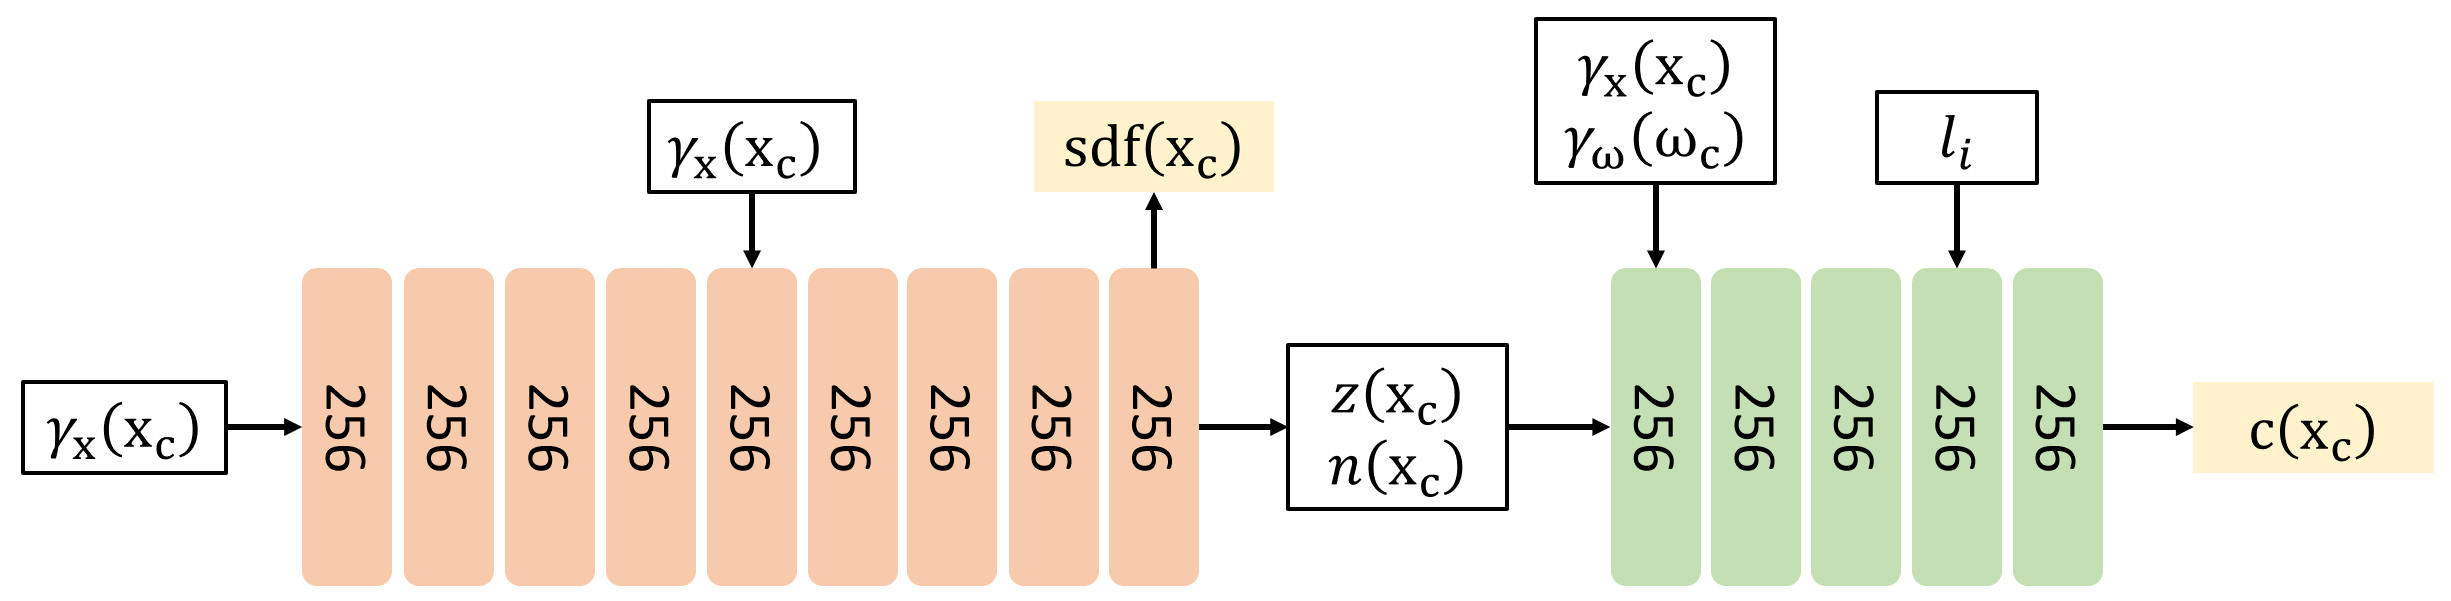
\includegraphics[width=0.7\linewidth]{./fig/net_geo.png}
\end{center}
\caption{Architecture of the geometry and color network.}
\label{fig:geo_net}
\end{figure*}

\begin{figure*}[t]
\begin{center}
   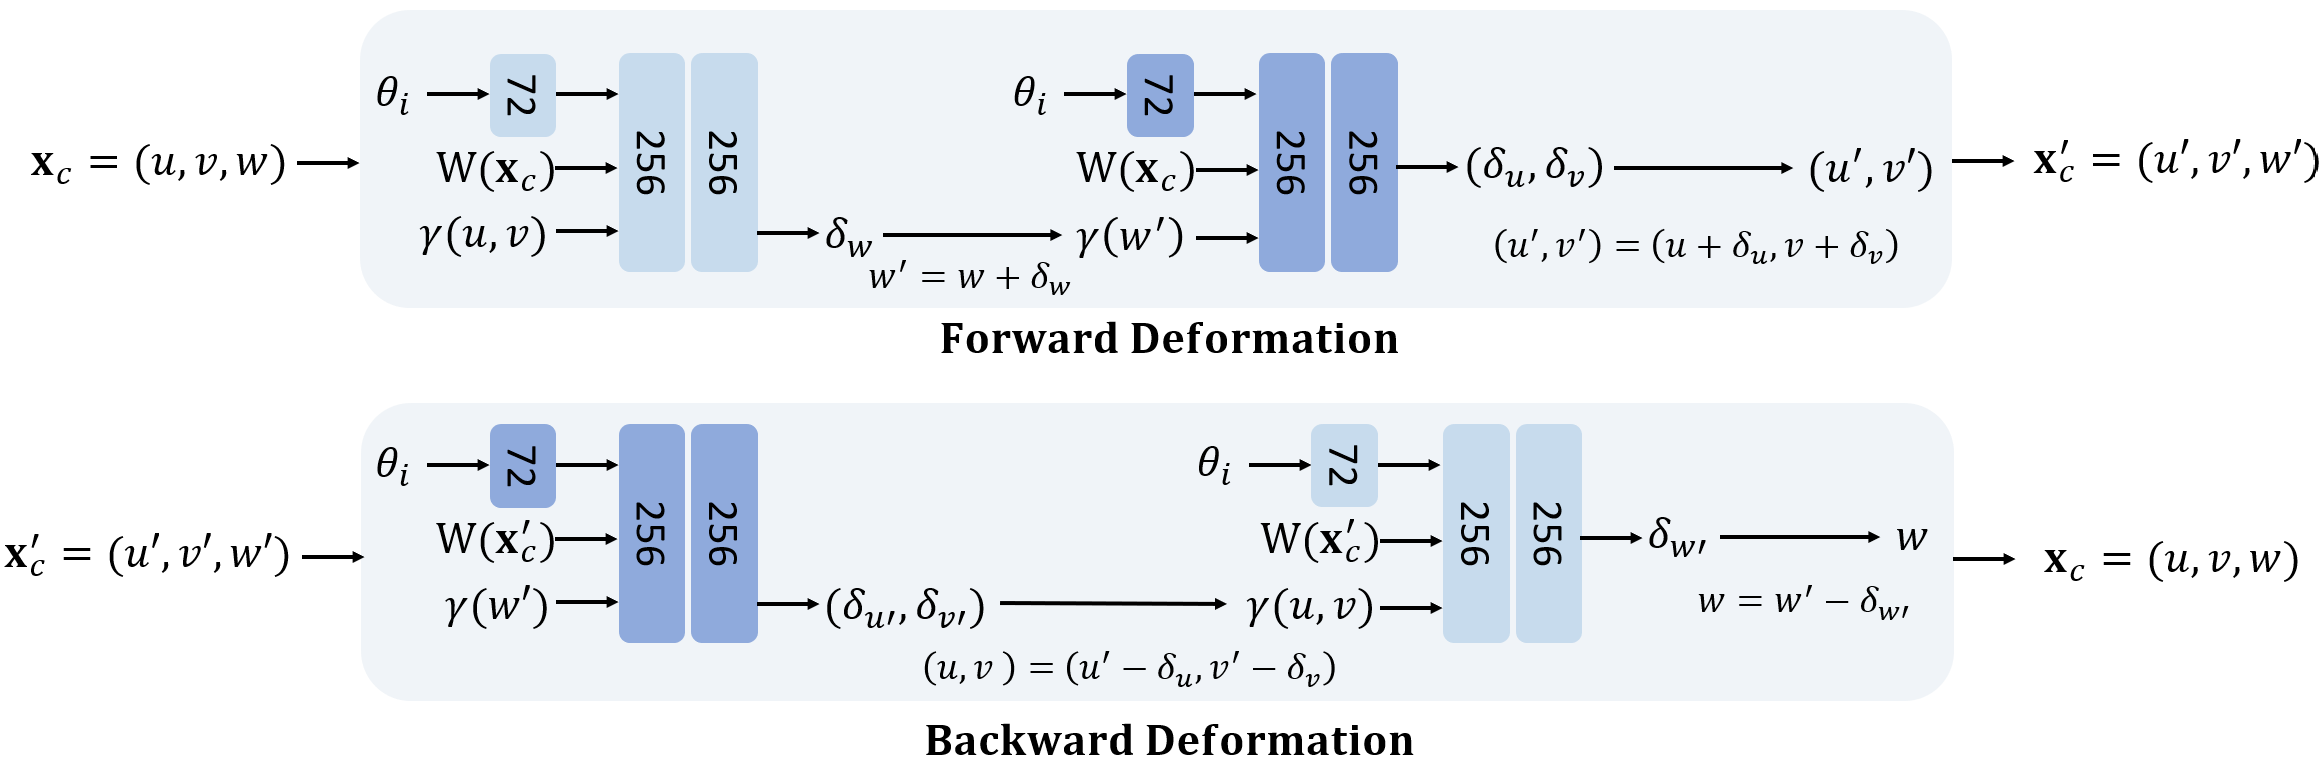
\includegraphics[width=0.85\linewidth]{./fig/net_def.png}
\end{center}
\caption{Architecture of the basic block in the invertible deformation network.}
\label{fig:def_net}
\end{figure*}

In this section, we provide more details about the network architectures, the training process and the used datasets.

\subsection{Network Architectures}

First, we show the structure of the geometry and color network used in the geometry and motion reconstruction stage, illustrated in Fig.~\ref{fig:geo_net}.
The orange part is the geometry network, the green part is the color network.
The $\gamma_\mathbf{x}(\cdot), \gamma_\mathbf{\omega}(\cdot)$ are the positional encoding functions for query points and view directions. 
The frequencies are 10 for positions, and 4 for directions, which is the same for all the neural networks in our method.
In Fig.~\ref{fig:geo_net}, $\mathbf{z}(\mathbf{x}_c)$ is the feature vector with a size of 256, $\mathbf{n}(\mathbf{x}_c)$ is the normal of $\mathbf{x}_c$, calculated through the gradient of the SDF field. Additionally, $l_i$ is the appearance latent code of the $i$th frame with a size of 128. 

Next, we show the basic transformation block of the invertible displacement network in Fig.~\ref{fig:def_net}, with the procedures for both forward and backward deformation. 
$\mathbf{W}(\mathbf{x}_c) \in \mathbb{R}^{24}$ is the skinning weights vector, $\gamma(\cdot)$ is the positional encoding function.
The full displacement network consists of 3 blocks, and $(u, v, w)$ are split in 3 different orders.

In the light visibility estimation module, each sub-network is an MLP with 3 hidden layers and a width of 128.
In the ablation study, the light visibility estimation network without part-wise design is an MLP with 4 hidden layers and 256 in width. It should be noted that the size of this network is the same as the light visibility network of Relighting4D~\cite{Relighting4D}.

In the material network $M$, the encoder is an MLP with 4 hidden layers and a width of 512, the dimension of the latent space is 32, and the decoder is an MLP with 2 hidden layers and a width of 128.
The roughness weights in $M$ contain 9 different specular bases defined by different roughness values. 

\subsection{Training Details}

For geometry and motion reconstruction, the loss weights are $\lambda_{\text{pixel}}=1, \lambda_{\text{mask}}=1, \lambda_{\text{eik}}=0.01, \lambda_{\text{disp}}=0.02$.
The $\mathcal{L}_{\text{mask}}$ term is implemented in a coarse to fine manner as in IDR \cite{idr}.
For a sampled ray $r$, we find the minimum SDF value $s_r$ along the ray and apply binary-cross-entropy loss as follow:
\begin{equation}
    \mathcal{L}_{\text{mask}} = \sum_{r\in \mathcal{R}} \text{BCE}\left(\text{sigmoid}(-\alpha s_r), M(r)\right)
\end{equation}
where $M(r) \in \{0, 1\}$ is the ground truth mask for the ray $r$, $\alpha$ is initially set to 50 and multiplied by a factor of 2 every 20 epochs. The number of multiplications of $\alpha$ is up to 5.

At the geometry and motion reconstruction stage, we train the network for 400 epochs. For the first 40 epochs, we use the posed SMPL \cite{loper2015smpl} mesh to compute the skinning weights in the observation space, and the output displacements are set to zero.
After this warm-up process, we replace the SMPL mesh with the extract body mesh, and use the displacement network to apply bidirectional deformations.
The body mesh is extracted from the canonical SDF field using marching cubes algorithm \cite{marchingcubes}.

For the training of the light visibility network, we sample 2000 poses from the AIST++ \cite{aist} dataset.
For each pose, we randomly sample 4 light directions and 16,384 3D points and compute their light visibility.
The networks are trained for 32 epochs.
Please note that the training and novel poses in Tab.~1 of the main paper are both unseen for the light visibility network. 
The training poses in the table are the poses seen in the input videos, and the novel poses are just used to evaluate the animatable capability.

At the material and lighting optimization stage, the loss weights are $\lambda_{\text{pixel}}=1, \lambda_{\text{kl}}=0.001, \lambda_{\text{smooth}}=0.01, \lambda_{\mathbf{z}}=1.0, \lambda_{\mathbf{x}}=0.05$.
The models are trained for 200 epochs.

During volume rendering, we first uniformly sample 256 points per ray.
For the geometry and motion reconstruction stage, we only keep the ray points close to the body mesh for color integration.
For the material and light estimation stage, as the trained geometry is fixed, the material network only needs to query the sampled points with non-zero weights for volumetric rendering.

We implement our model using PyTorch and use the Adam \cite{adam} optimizer for training.
The learning rate is $5e-4$ for the first and third stages and $1e-3$ for the second stage.
All the models are trained on a single NVIDIA RTX 3090 GPU.
It takes about a day each to train the first and third stages, and the light visibility estimation network takes approximately 12 hours to train.

During inference, our method with the part-wise visibility network takes about 40s to render an image of $512\times512$ resolution. 
Besides, it takes about 18s and 22s for our method without the visibility network and with a single visibility network respectively. 
The additional time for querying 15 body parts for light visibility is acceptable and the part-wise light visibility module achieves significantly better results than the single network.
In contrast, computing light visibility through ray tracing takes about 430s per frame, causing the training of the network to be more than 10 days. 

\subsection{Dataset Details}
Here we provide more details about the used datasets.
For the synthetic dataset, we synthesize 4 body motion sequences as the training set, each containing 100 frames.
We sample 10 frames evenly from each sequence for evaluation.
For the novel pose evaluation, we sample 10 out-of-distribution poses from the AIST++ \cite{aist} dataset.
The videos in the dataset are generated under 8 different views, with 4 views used for training and the other 4 views used for evaluation. 

For evaluation on real datasets, we follow the data preprocessing method and the training-test split of \citet{peng2022animatable} for the ZJU-MoCap \cite{neuralbody}, Human3.6M \cite{h36m}, DeepCap \cite{deepcap} and PeopleSnapshot \cite{alldieck2018video} datasets.
In our experiments, there are 4 input views used in the ZJU-MoCap and DeepCap datasets, 3 input views used in the Human3.6M dataset, and a single input view used in the PeopleSnapshot dataset. 
In the ZJU-MoCap, DeepCap and PeopleSnapshot datasets, the number of frames in the input videos is 300.
In the Human3.6M dataset, the number of training frames ranged from 150 to 260.

\section{Evaluation of the Deformation Cycle Consistency}

We propose an invertible deformation field that allows for bidirectional deformation while maintaining cycle consistency.
For ordinary invertible neural networks, the cycle consistency is strictly satisfied.
However, we involve the skinning weights $\mathbf{W}(\mathbf{x})$ as an additional condition of the deformation network to improve the geometry reconstruction results, which slightly sacrifices the cycle consistency of the deformation field.
In this section, we evaluate the cycle consistency of the proposed invertible deformation network.

To evaluate the cycle consistency, we first sample some points on the body mesh.
Then for a sampled point $\mathbf{x}$, we apply the forward displacement $f(\mathbf{x})$ to obtain the deformed point $\mathbf{x}' = \mathbf{x} + f(\mathbf{x})$.  
Then, we apply the backward displacement $f^{-1}(\mathbf{x}')$ to $\mathbf{x}'$ to obtain the final transformed point $\mathbf{x}'' = \mathbf{x'} + f^{-1}(\mathbf{x}')$.
The goal is for $\mathbf{x}''$ to be close to $\mathbf{x}$, indicating that the forward and backward deformations are consistent.
We use the relative deformation error as the metric:
\begin{equation}
    \mathcal{L} = \frac{2 \|\mathbf{x}'' - \mathbf{x}\|_2} {\|\mathbf{x}' - \mathbf{x}\|_2 + \|\mathbf{x}'' - \mathbf{x}'\|_2}
\end{equation}

We compare our invertible network with the single directional deformation network of \citet{peng2022animatable}, which is a 9 hidden layer, 256 width MLP.
For the single directional MLP, we assume that the backward deformation is simply the negative of the forward deformation: $f^{-1}(\mathbf{x}) = -f(\mathbf{x})$.
We find that the average deformation error of the single directional MLP is $9.45\%$, while the deformation error of our invertible network is only $1.66\%$.
This indicates that our network is significantly better at maintaining cycle consistency. 

\section{Correspondence Visualization}
We show the estimated correspondences in Fig.\ref{fig:corres}, the results correspond to Fig.\ref{fig:geo_artifact}.
The left part shows the overlay between the mesh and the image and the right part shows the correspondences between the canonical space and the observation space, where color encodes the correspondences. 
Since the explicit mesh fits the body surface well, the computed inverse skinning weights find better correspondences between the canonical and observation spaces, and using only SMPL will lead to artifacts due to the miss matches as shown in the results of ``Ours w/o MIS".
Besides, the correspondences of other methods also mix the arms with the body. 

\begin{figure*}[t]
\begin{center}
   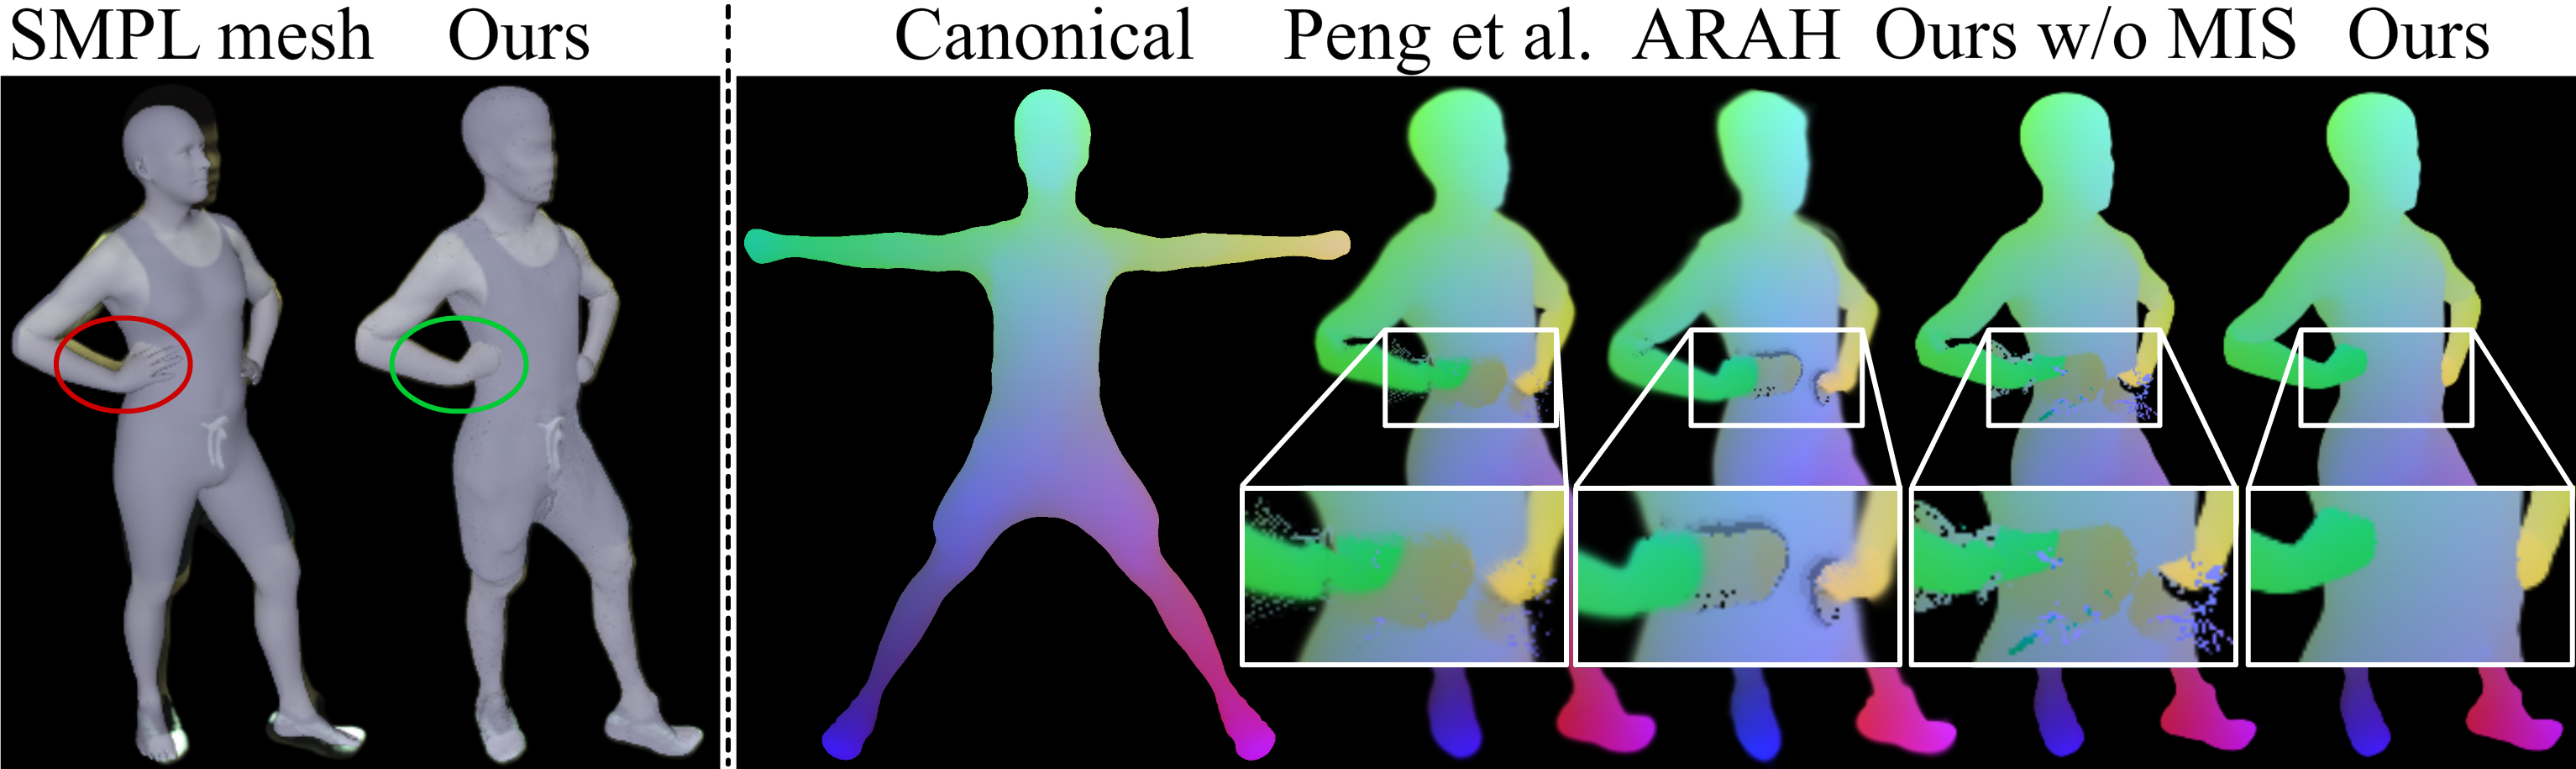
\includegraphics[width=0.65\linewidth]{./fig/corres_zoom_in.jpg}
\end{center}
\caption{Visualization of estimated correspondences.}
\label{fig:corres}
\end{figure*}

\begin{figure}[t]
\begin{center}
   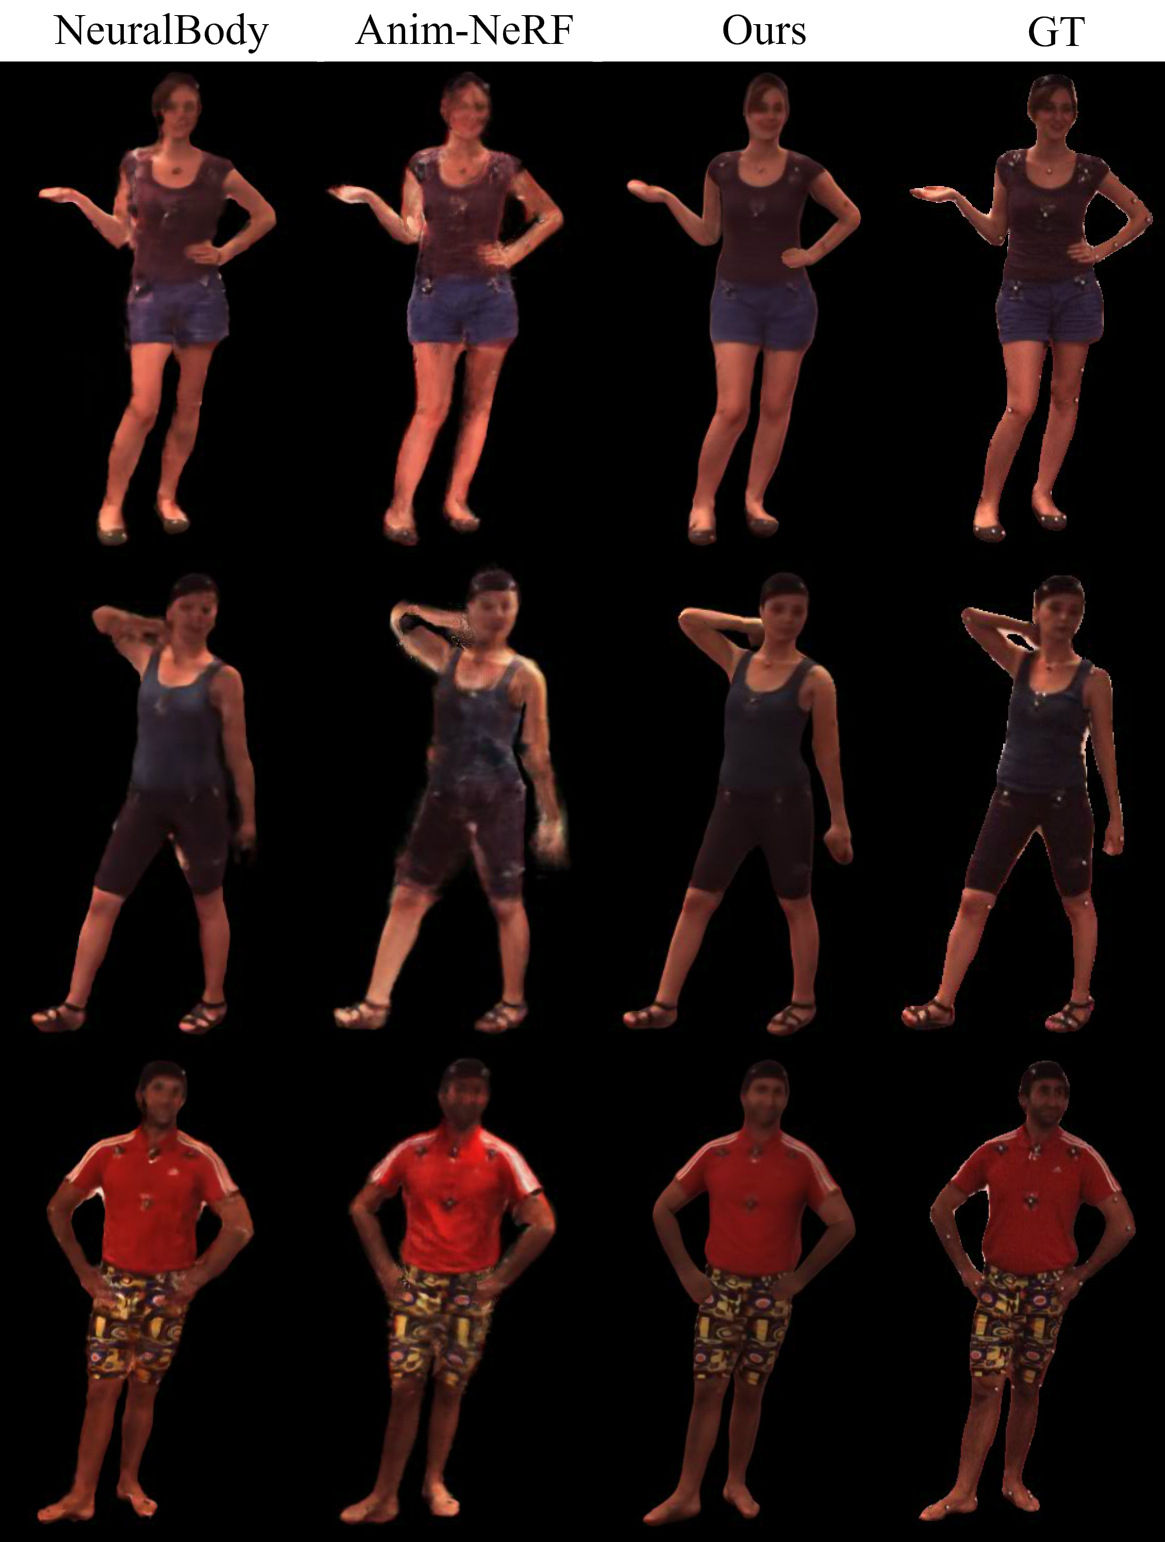
\includegraphics[width=1.0\linewidth]{./fig/h36m.jpg}
\end{center}
\caption{Qualitative comparisons of novel pose synthesis on the Human3.6M dataset.}
\label{fig:h36m}
\end{figure}

\section{Comparisons with Non-relightable Methods}
In this section, we compare our method with state-of-the-art non-relightable methods on the Human3.6M \cite{h36m} dataset for novel view and novel pose synthesis.
We follow the test split of Anim-NeRF \cite{animatablenerf} and show quantitative results of novel view and novel pose synthesis in Tab.~\ref{tab:non-relit-sp} and Tab.~\ref{tab:non-relit-np} respectively.
The numerical results of these methods come from the recent work NPC \cite{su2023npc}.
We can see that our method achieves comparable results with state-of-the-art non-relightable methods and our results are better than NeuralBody \cite{neuralbody}, Anim-NeRF \cite{animatablenerf} and A-NeRF \cite{a-nerf}.
Note that these non-relightable methods directly predict view-dependent color, while the results of our method are rendered with the reconstructed material and lighting. 
So the results of these methods cannot be relight under novel scenes like ours.
We further show qualitative comparisons of novel pose synthesis with NeuralBody \cite{neuralbody} and Anim-NeRF \cite{animatablenerf} in Fig.~\ref{fig:h36m}.
Our method achieves better visual quality than the other two methods.


\begin{table*}[t]
\begin{center}
\scalebox{0.85}{
\begin{tabular}{cccccccccc}
\hline
\multirow{2}{*}{Method} & \multicolumn{3}{c}{S1} & \multicolumn{3}{c}{S5} & \multicolumn{3}{c}{S9} \\
                        & PSNR$\uparrow$ & SSIM$\uparrow$ & LPIPS$\downarrow$ & PSNR$\uparrow$ & SSIM$\uparrow$ & LPIPS$\downarrow$ & PSNR$\uparrow$ & SSIM$\uparrow$ & LPIPS$\downarrow$  \\
\hline
NeuralBody \cite{neuralbody} & 22.88 & 0.897 & 0.139 & 24.61 & 0.917 & 0.128 & 24.29 & 0.911 & 0.122\\
Anim-NeRF \cite{animatablenerf} & 22.74 & 0.896 & 0.151 & 23.40 & 0.895 & 0.159 & 24.86 & 0.911 & 0.145\\
A-NeRF \cite{a-nerf} & 23.93 & 0.912 & 0.118 & 24.67 & 0.919 & 0.114 & 25.58 & 0.916 & 0.126 \\
ARAH \cite{ARAH} & 24.53 & 0.921 & 0.103 & 24.67 & 0.921 & 0.115 & 25.43 & 0.924 & 0.112 \\
DANBO \cite{danbo} & 23.95 & 0.916 & 0.108 & 24.86 & 0.924 & 0.108 & 26.15 & 0.925 & 0.108 \\
TAVA \cite{tava} & \textbf{25.28} & \textbf{0.928} & 0.108 & 24.00 & 0.916 & 0.122 & 26.20 & 0.923 & 0.119 \\
NPC \cite{su2023npc} & 24.81 & 0.922 & \textbf{0.097} & \textbf{24.92} & \textbf{0.926} & \textbf{0.100} & \textbf{26.39} & \textbf{0.930} & \textbf{0.095} \\
\hline
Ours & 24.45 & 0.910 & 0.115 & 24.59 & 0.911 & 0.119 & 26.24 & 0.920 & 0.111 \\
\hline
\end{tabular}
}
\caption{Novel-view synthesis comparisons on the Human3.6M dataset.}
\label{tab:non-relit-sp}
\end{center}
\end{table*}

\begin{table*}[t]
\begin{center}
\scalebox{0.85}{
\begin{tabular}{cccccccccc}
\hline
\multirow{2}{*}{Method} & \multicolumn{3}{c}{S1} & \multicolumn{3}{c}{S5} & \multicolumn{3}{c}{S9} \\
                        & PSNR$\uparrow$ & SSIM$\uparrow$ & LPIPS$\downarrow$ & PSNR$\uparrow$ & SSIM$\uparrow$ & LPIPS$\downarrow$ & PSNR$\uparrow$ & SSIM$\uparrow$ & LPIPS$\downarrow$  \\
\hline
NeuralBody \cite{neuralbody} & 22.10 & 0.878 & 0.143 & 23.52 & 0.897 & 0.144 & 23.05 & 0.885 & 0.150 \\
Anim-NeRF \cite{animatablenerf} & 21.37 & 0.868 & 0.167 & 22.29 & 0.875 & 0.171 & 23.73 & 0.886 & 0.157 \\
A-NeRF \cite{a-nerf} & 22.67 & 0.883 & 0.159 & 22.96 & 0.888 & 0.155 & 24.16 & 0.889 & 0.164 \\
ARAH \cite{ARAH} & 23.18 & 0.903 & 0.116 & 22.91 & 0.894 & 0.133 & 24.15 & 0.896 & 0.135 \\
DANBO \cite{danbo} & 23.03 & 0.895 & 0.121 & \textbf{23.66} & 0.903 & 0.124 & 24.79 & 0.904 & 0.130 \\
TAVA \cite{tava} & \textbf{23.83} & \textbf{0.908} & 0.120 & 22.89 & 0.898 & 0.135 & 24.80 & 0.901 & 0.138 \\
NPC \cite{su2023npc} & 23.39 & 0.901 & \textbf{0.109} & 23.63 & \textbf{0.906} & \textbf{0.113} & 24.86 & \textbf{0.907} & \textbf{0.115} \\
\hline
Ours & 23.25 & 0.890 & 0.127 & 23.39 & 0.894 & 0.132 & \textbf{25.05} & 0.900 & 0.131 \\
\hline
\end{tabular}
}
\caption{Novel-pose synthesis comparisons on the Human3.6M dataset.}
\label{tab:non-relit-np}
\end{center}
\end{table*}

\begin{figure*}[t]
\begin{center}
   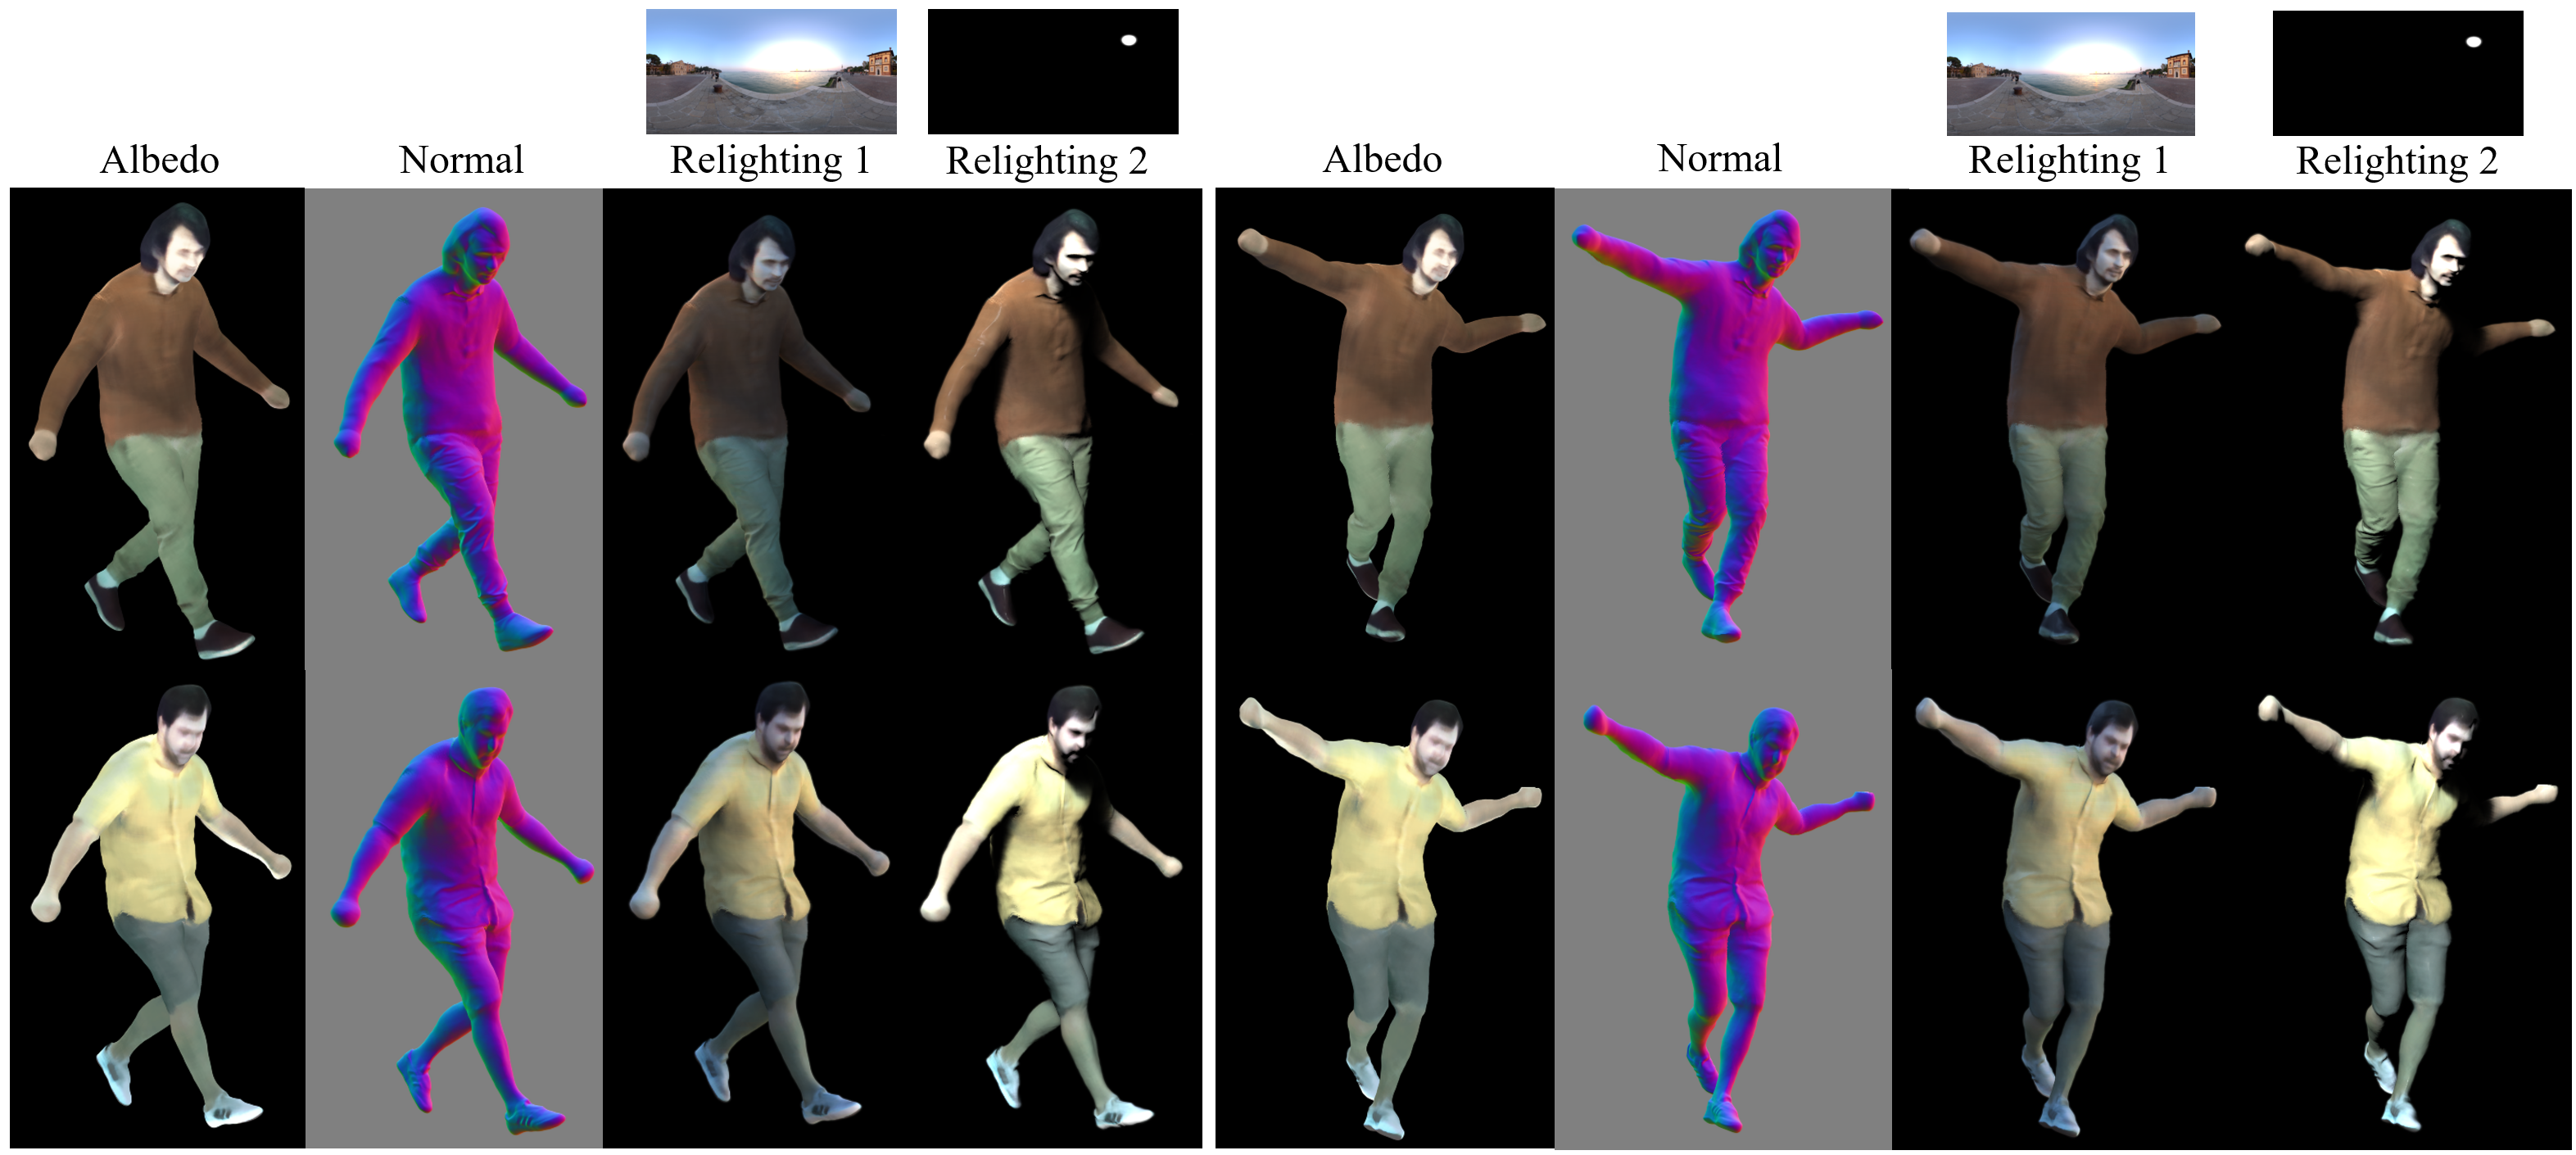
\includegraphics[width=1.0\linewidth]{./fig/deepcap.png}
\end{center}
\caption{Results of our technique on the DeepCap dataset. From left to right of each result: the albedo of an animated pose, the corresponding normal in this pose, and two relighting results. }
\label{fig:deepcap}
\end{figure*}

\begin{figure*}[t]
\begin{center}
   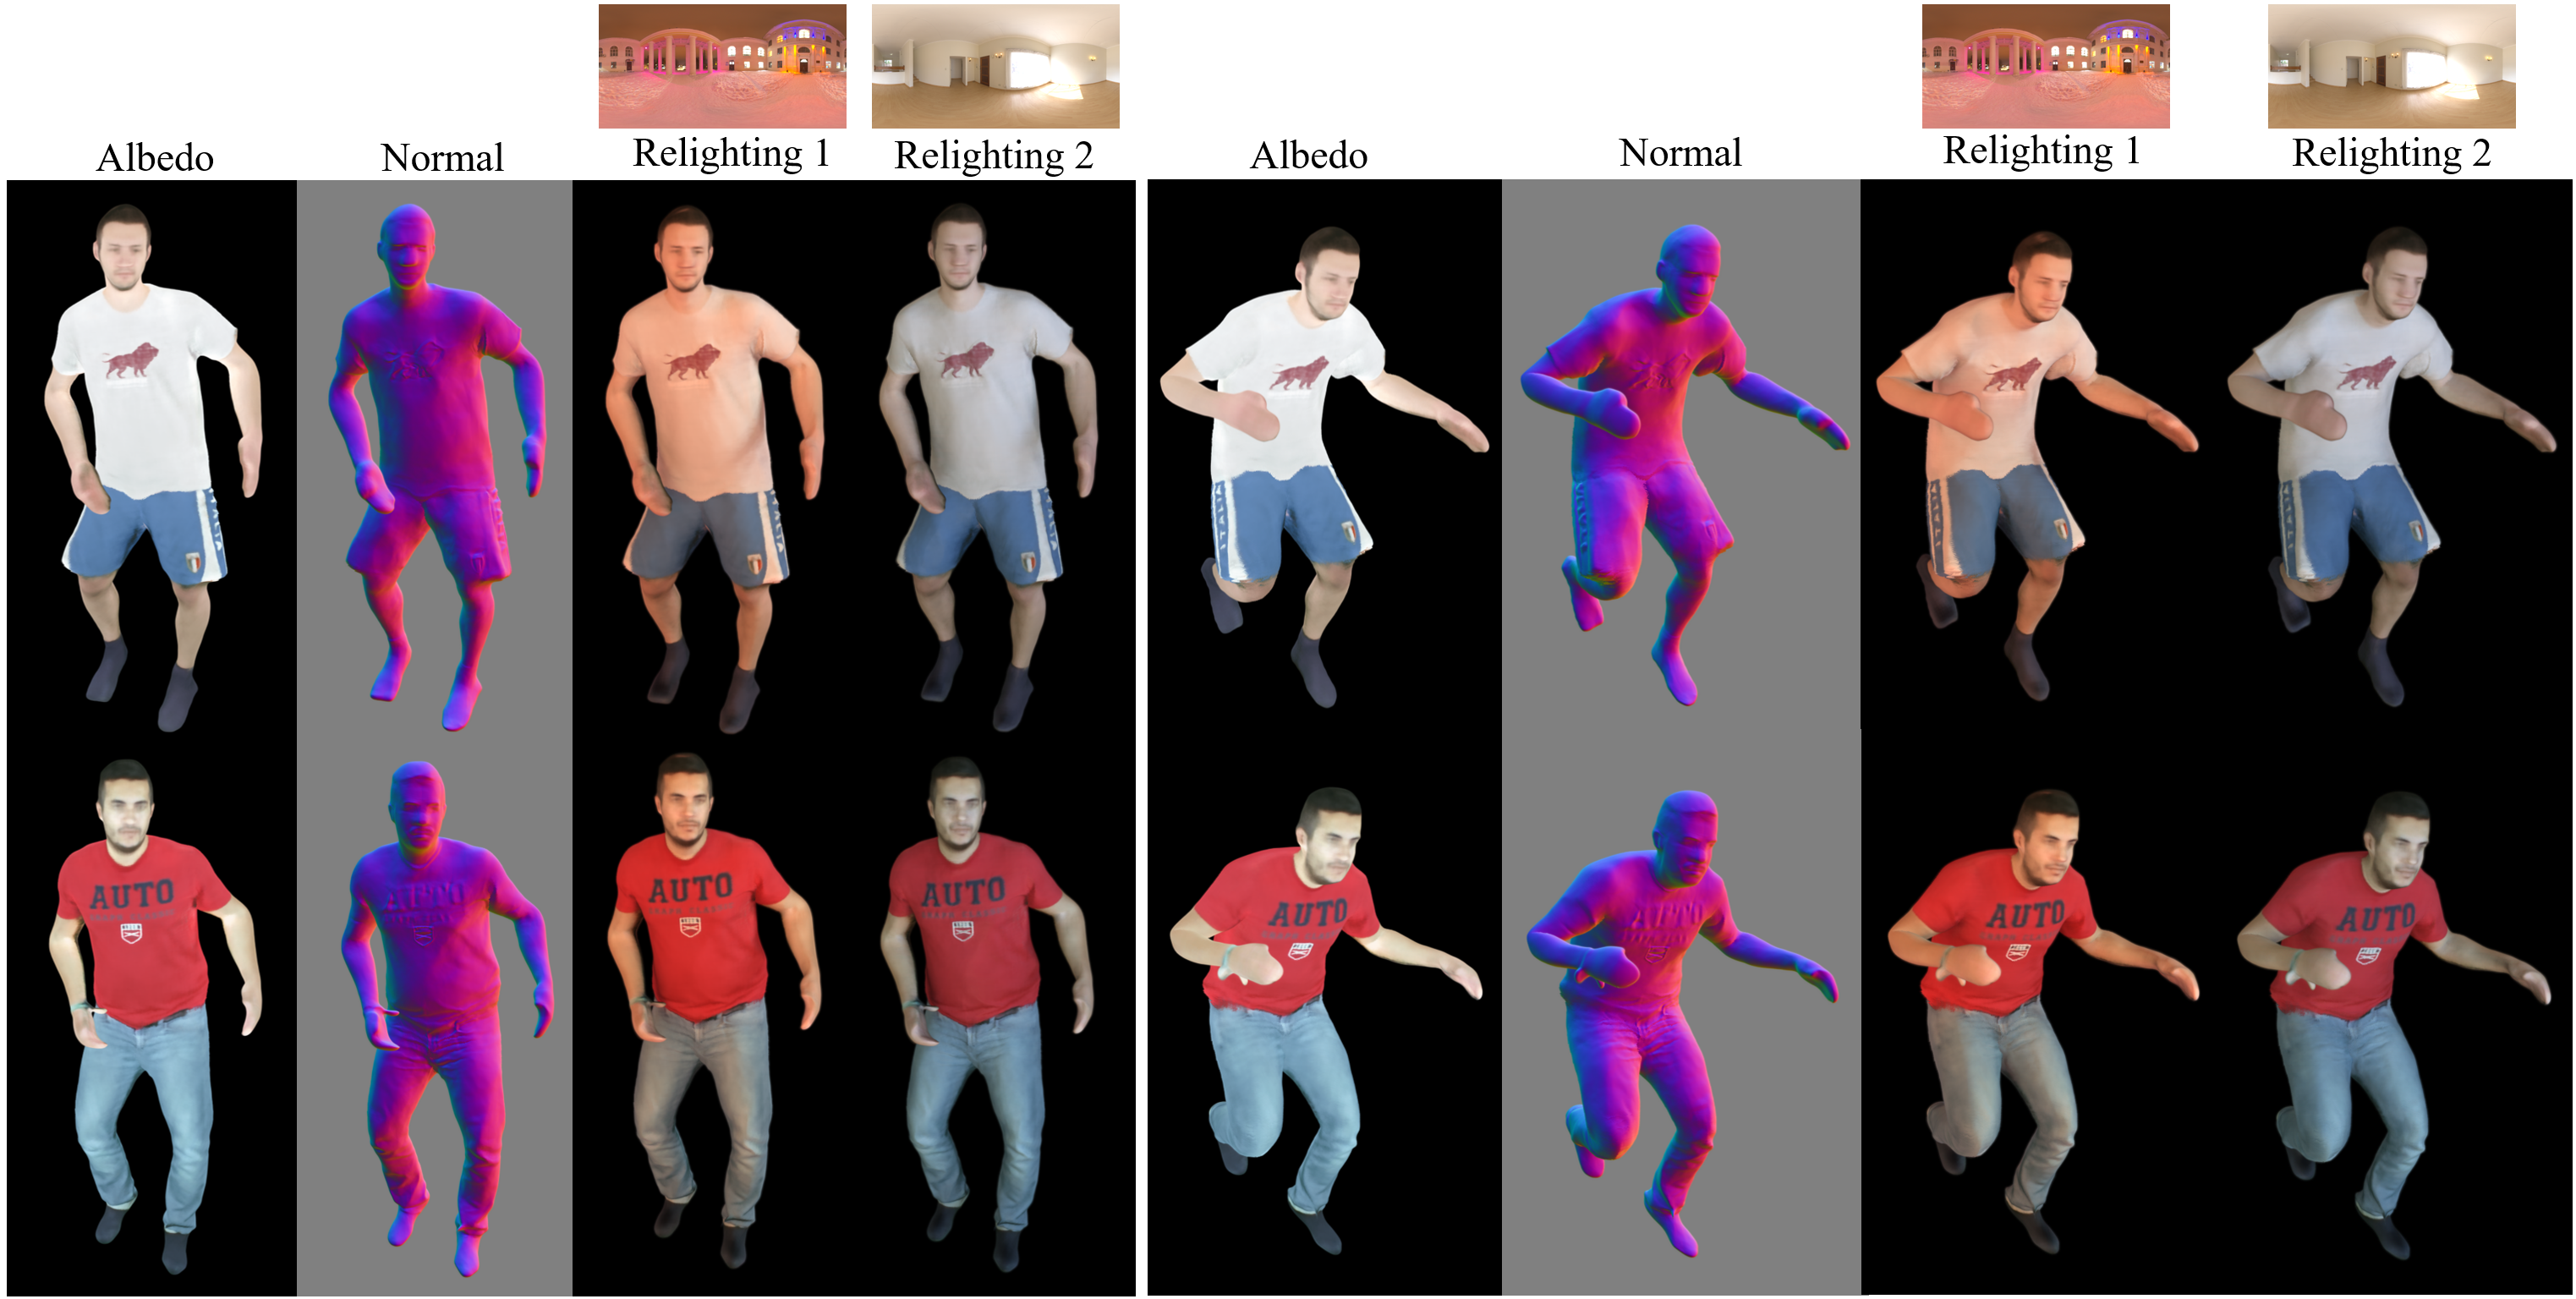
\includegraphics[width=1.0\linewidth]{./fig/peoplesnap.png}
\end{center}
\caption{Results of our technique on the PeopleSnapshot dataset. From left to right of each result: the albedo of an animated pose, the corresponding normal in this pose, and two relighting results. }
\label{fig:ps}
\end{figure*}

\begin{figure*}[t]
\begin{center}
   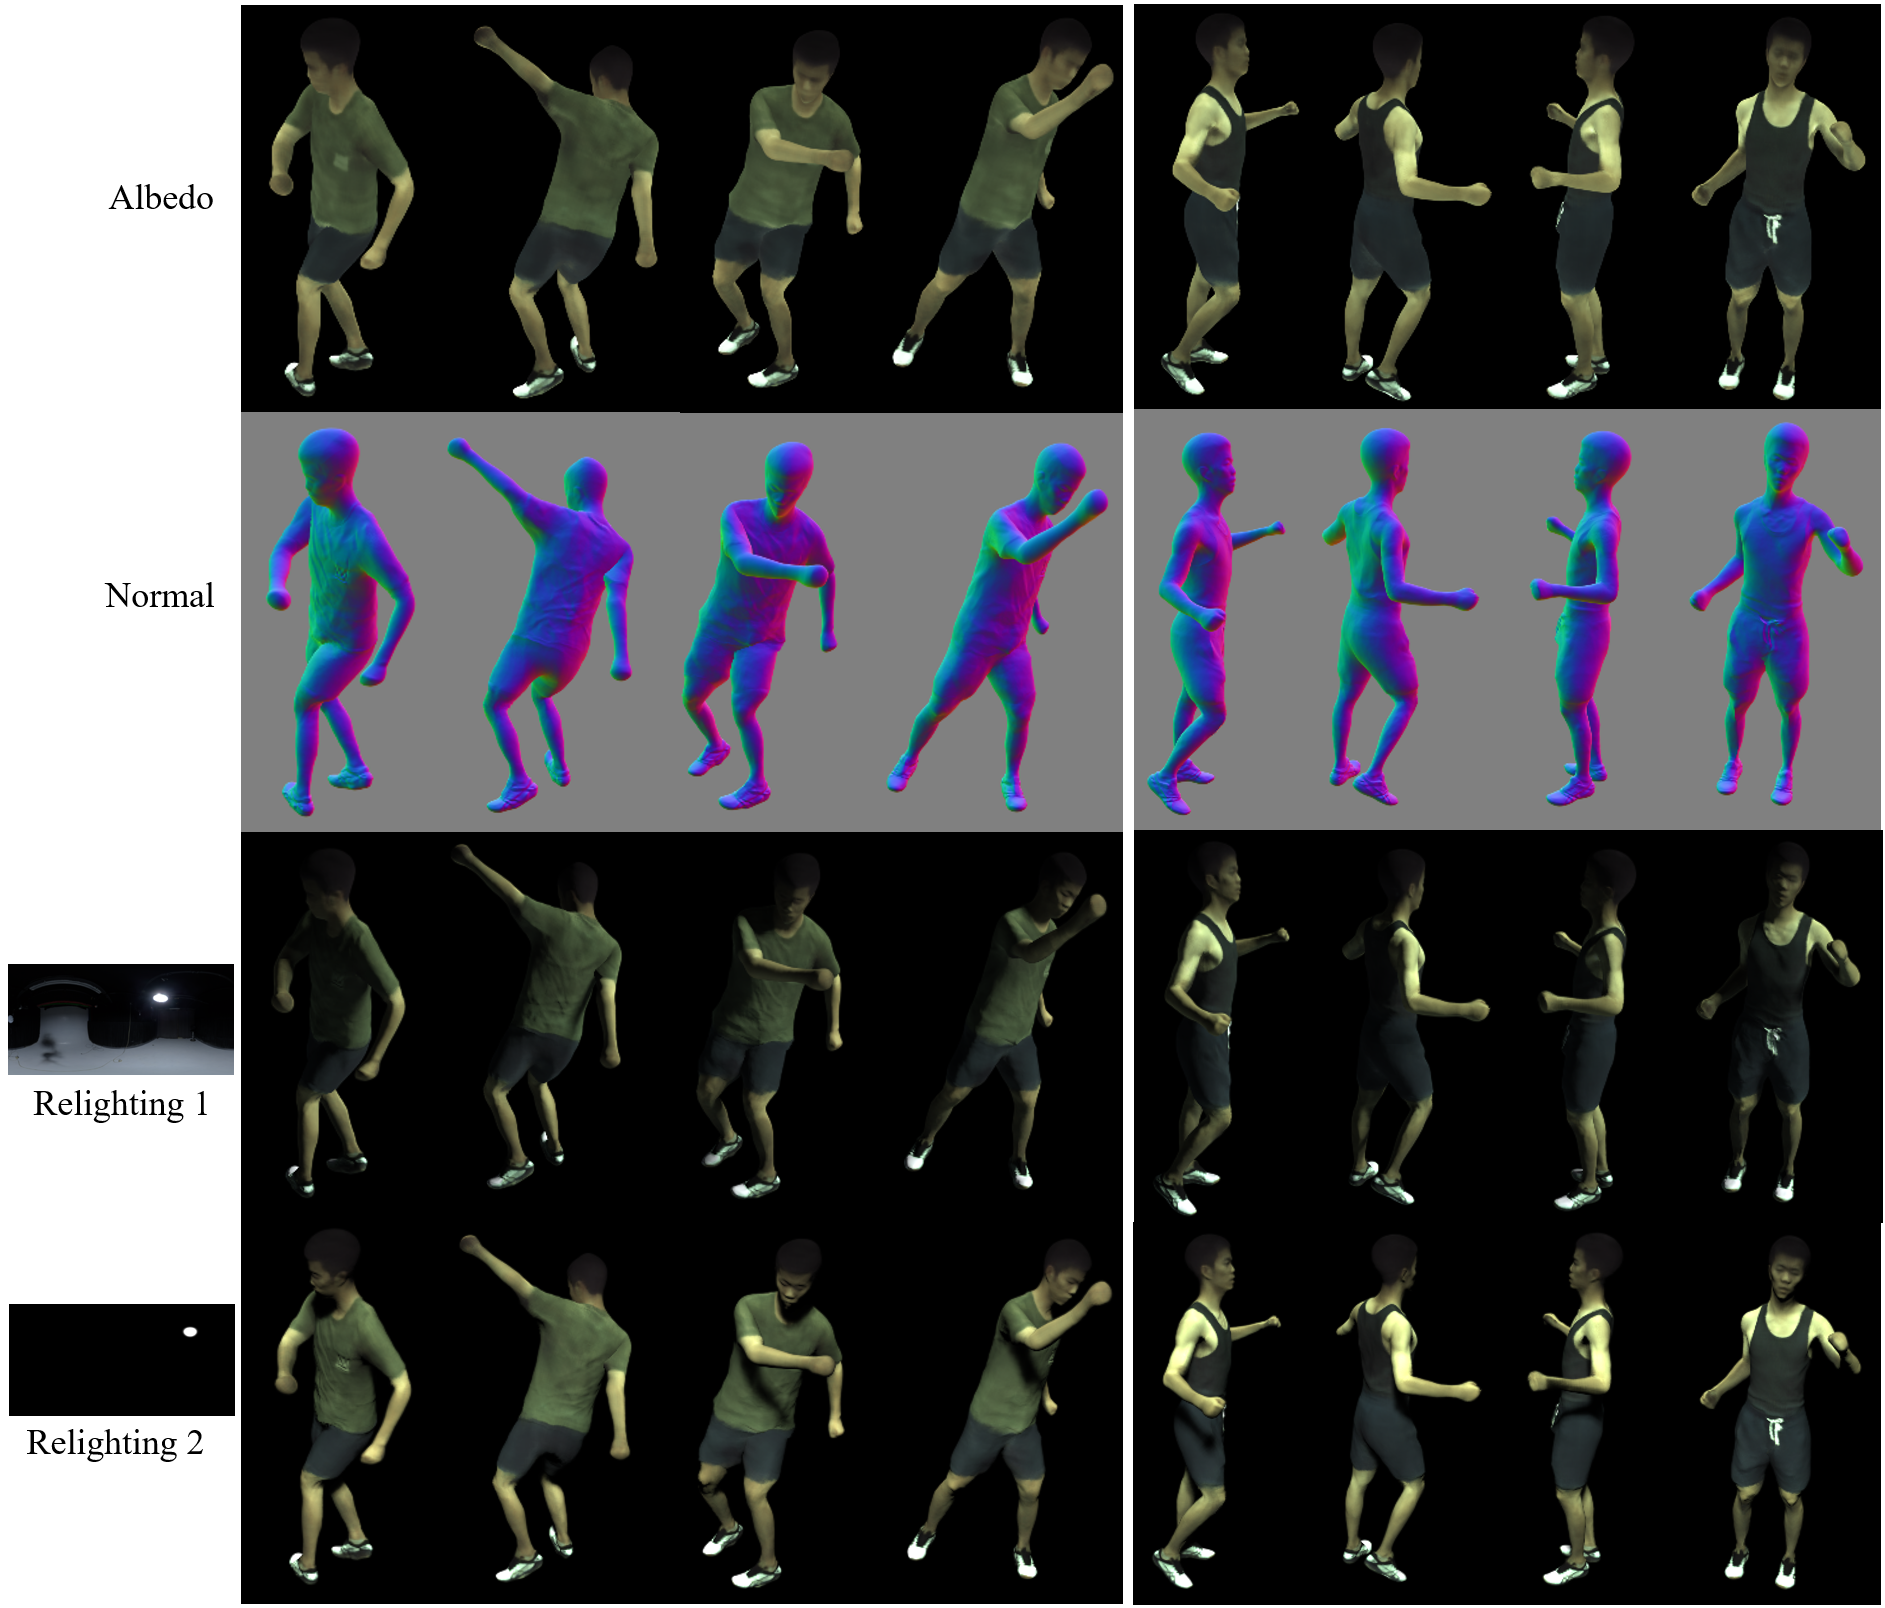
\includegraphics[width=0.90\linewidth]{./fig/single_view.png}
\end{center}
\caption{Results on the ZJU-MoCap dataset with single-view input. From top to bottom: the reconstructed albedo, normal of the reconstructed geometry, and two relighting results.}
\label{fig:single_view}
\end{figure*}

\section{More Results}
In this section, we present more results of our method.
First, we show results on the DeepCap \cite{deepcap} dataset in Fig.~\ref{fig:deepcap}.
Note that our method also reconstructs geometry details like cloth wrinkles as shown in the normal maps. 
Besides, our method also works well with only single-view videos as input, we show the results of our method on the PeopleSnapshot \cite{alldieck2018video} dataset in Fig.~ \ref{fig:ps}.
Moreover, our method also produces plausible results on the ZJU-MoCap \cite{neuralbody} dataset with single input view, as shown in Fig.~\ref{fig:single_view}.
The input monocular videos from the ZJU-MoCap dataset contain 500 frames.
Note that these subjects from different datasets are captured under different lighting conditions, indicating that our method is robust to different shooting environments. 
For video results, please refer to the supplemental video.